\documentclass[a4paper, oneside, 12pt]{book}
\usepackage [spanish] {babel}
\usepackage [latin1] {inputenc}
\usepackage [pdftex]{graphicx}
\usepackage {listings}
\usepackage {times}


%Este archivo contiene las definiciones de los m�rgenes,
%espaciados etc...
%En la normativa se define que el margen izquierdo debe
%ser de 35 mm. Tener en cuenta que en LaTeX hay un comando
%para definir la distancia del borde del papel respecto
%a las notas al margen (que no se usan en los proyectos y
%cuya longitud est� en \evensidemargin y/o \oddsidemargin)
%y hay otro comando distinto para indicar el margen
%desde el borde de salida al cuerpo del texto, que es
%lo que modificamos aqui

\setlength\oddsidemargin{0cm}
\setlength\marginparwidth{3.5cm}




%El margen derecho debe ser 2cm. Como A4 mide 21 cm
%de ancho y dado que ya hemos consumido 3.5cm por la
%izquierda, la anchura del texto en las p�ginas debe
%ser de 21-3.5-2=15.5
\setlength\textwidth{15.5cm}

%La sangr�a a principio de l�nea
\setlength\parindent{1.5cm}

\begin {document}


%Falta por componer la portada del proyecto!!!


%Primer p�gina del proyecto
\begin{titlepage}
	
\begin{center}

%Logotipo de la Escuela
\begin{figure}
	\centering
		
\includegraphics[width=0.20\textwidth]{figuras/png/esi_flat.png}
	\label{fig:esi_flat}
\end{figure}

\vfill
			\Large\textbf{UNIVERSIDAD DE CASTILLA-LA MANCHA}

						

						\textbf{ESCUELA SUPERIOR DE INFORM�TICA}

													

						\vfill
							DEPARTAMENTO DE INGENIER�A EL�CTRICA, ELECTR�NICA
							Y AUTOM�TICA
						\vfill

									PROYECTO FIN DE CARRERA



\textbf{SimProc: Un simulador gr�fico de procesos secuenciales automatizados}
\vfill
\begin{flushleft}
Autor: �scar G�mez Garc�a

Director: Jes�s Salido Tercero
\end{flushleft}

\vfill

\begin{flushright}
\textbf{Septiembre, 2006}
\end{flushright}
\end{center}

\end{titlepage}
%Fin de la pagina de PORTADA


%Indicamos al paquete listings que el lenguaje usado es C++
\lstset{language=C++,
	basicstyle=\small, 
	showstringspaces=false,
	frame=single}
\tableofcontents
\subsection {Introducci�n}

En este apartado se define el dise�o del sistema en t�rminos de paquetes, clases, interrelaciones y comportamiento. Se utilizar�n diagramas UML para mostrar aspectos espec�ficos a destacar en el dise�o global del sistema como el dise�o de la interfaz de usuario o el dise�o estructural.

Existen algunos detalles importantes que un desarrollador deber�a conocer a la hora de entender, modificar o ampliar el dise�o sugerido:

\begin {itemize}

\item {La arquitectura global de la aplicaci�n est� basada en el patr�n Modelo-Vista-Control. Este patr�n muestra la soluci�n m�s cl�sica y eficaz para el desarrollo de una aplicaci�n interactiva separando claramente los componentes m�s elementales: Los datos que maneja la aplicaci�n (el ``Modelo''), los mecanismos que implementan la l�gica de control (el ``Controlador'' y el c�digo de la interfaz de usuario (la ``Vista'').}
\item {El Modelo no est� desarrollado mediante un lenguaje de programaci�n cl�sico, sino que consiste en la definici�n de un vocabulario XML que declara los componentes b�sicos necesarios para la automatizaci�n de un proceso, como por ejemplo rel�s, motores e interruptores.}
\item {El vocabulario del Modelo se especifica en un documento XML que contiene una definici�n escrita en XML Schema y donde se define la sintaxis que debe tener un modelo de sistema automatizado. La comprensi�n de la sintaxis del Schema puede resultar dif�cil para un desarrollador que se aproxime a ella por primera vez por lo que se recomienda leer la especificaci�n del World Wide Web Consortium para XML Schemas que se documenta en INSERTAR-----REFERENCIA----AQUI----- }
\item {El Controlador ha sido escrito en C++ est�ndar de forma que existe una correspondencia estricta entre los elementos definidos en el esquema y las clases que implementan un sistema. As� para cada elemento at�mico del esquema existe una clase que lo implementa.}
\item {Mantener la correspondencia entre una implementaci�n C++ y un documento XML que la represente es una tarea de gran complejidad. Por ello se ha utilizado Xerces, un framework escrito en C++ que implementa fielmente las recomendaciones del W3C para XML. Xerces posee implementaciones en C++ y Java, ademas de disponer de proyectos de implementaci�n en lenguajes alternativos.En ��INSERTAR REFERENCIA TUTORIAL WXWIDGETS AQUI!! se ilustra el uso de Xerces en un programa.}
\item {La Vista se ha implementado utilizando WxWidgets, un conjunto de clases multiplataforma para la escritura de interfaces de usuario altamente portable y con un aspecto diferenciado para los distintos sistemas de escritorio. La utilizaci�n de WxWidgets tambi�n presenta numerosas dificultades para un no iniciado por lo que su uso se describe con mayor amplitud en INSERTAR AQUI REFERENCIA TUTORIAL WXWIDGETS!!}
\item {La programaci�n del an�lisis de ficheros XML se puede hacer desde cero o utilizando las implementaciones de las recomendaciones del W3C. Estas recomendaciones especifican dos grandes enfoques de la programaci�n para XML, a saber: DOM y SAX. En este proyecto se ha utilizado la implementaci�n DOM de Xerces escrita en C+++}

\end {itemize}

El dise�o del software se ha centrado en la consecuci�n de una serie de objetivos:
\begin {itemize}
\item {Correcci�n: se pretende que el dise�o permita construir un programa que satisfaga los requisitos especificados.}
\item {Inteligibilidad: el dise�o no solamente es f�cil de transformar en una implementaci�n software sino que mediante el uso de patrones software deber�a ser f�cilmente comprensible para distintas personas que pretenden modificar o ampliar el sistema.}
\item {Modular: se ha intentado separar en capas los distintos aspectos concernientes a la implementaci�n de forma que las modificaciones supongan un impacto m�nimo, o al menos peque�o, en los distintos m�dulos.}
\item {Extensible: el uso de est�ndares bien conocidos as� como el aislamiento del c�digo en distintas capas debe facilitar la ampliaci�n del programa.}

\end {itemize}
\chapter {Objetivos}
\chapter {Estado de la cuesti�n}
\section {Herramientas de simulaci�n}
\section {Los lenguajes extensibles}

\subsection {Los formatos de almacenamiento cl�sicos}

En los primeros sistemas inform�ticos, las capacidades de almacenamiento eran muy limitadas, por lo que ni siquiera se conceb�a la idea de almacenar nada que no fuera lo que conocemos como texto plano. Adem�s, las limitadas capacidades de c�mputo as� como el limitado espacio tanto en discos como en memorias, hac�a totalmente inviable el uso de nada que no fueran caracteres.
A medida que los microprocesadores mejoraban y con el crecimiento del espacio disponible en disco y en memoria, empezaron a aparecer programas que no utilizaban el texto como su formato de almacenamiento sino que empezaron a utilizar archivos binarios, en lugar de los archivos de texto tan populares hasta ese momento. Por ejemplo podemos citar:

\begin {itemize}
\item {Los programas de tratamiento de texto que empezaron a incorporar la posibilidad de incorporar im�genes.}
\item {Los programas de proceso gr�fico que hab�an empezado a hacerse visibles al mercado dom�stico.}
\item {Entornos de desarrollo integrado que permit�an acercar el desarrollo de software al gran p�blico.}
\end {itemize}

El uso de archivos binarios supone que el almacenamiento de informaci�n ya no se hace en texto ``legible'' sino en forma de una secuencia de bits comprensible solamente para el programa que lo cre�. El uso de archivos binarios permiti� que dichos archivos ocuparan menos espacio (por ejemplo, incluyendo un archivo de imagen tal cual, en lugar mediante codificaci�n Base64) y permit�a que los programas trabajaran m�s deprisa, ya que en general, las codificaciones binarias son m�s eficientes.

Se puede decir a grandes rasgos que todos estos programas empezaron lo que supuso una revoluci�n para dos sectores muy claramente diferenciados:

\begin {itemize}

\item {Por un lado, los usuarios vieron como las posibilidades se multiplicaban y se empez� a demandar m�s y m�s. V�ase el caso de los procesadores de texto que permiten no ya la inclusi�n de gr�ficos, sino tambi�n de audio e incluso de v�deo.}
\item {Por otro lado, a la misma velocidad que las posibilidades del usuario crec�an, crec�an los problemas para desarrolladores de aplicaciones que intentaban que los formatos de almacenamiento de sus programas fueran comprensibles para otros programas, o incluso entre distintas versiones. }
\end {itemize}
\subsection {Los primeros lenguajes de marcas}

A pesar de que los formatos de almacenamiento binarios gozaban de ventajas tales como su reducido tama�o o la eficiencia de su procesamiento, r�pidamente se observ� que los ficheros de texto pose�an otra cualidad muy interesante: Eran legibles por parte de todos los programas con relativa facilidad, e incluso en ciertos casos, comprensible por las personas.

Esta cualidad fue la que llev� al desarrollo de un mecanismo que permitiera almacenar la informaci�n en forma de texto, pero a la vez permitiendo la existencia de datos binarios. Este mecanismo de almacenamiento qued� plasmado en SGML, un lenguaje que defin�a un formato de almacenamiento basado fundamentalmente en texto, pero que inclu�a la definici�n de marcas que daban informaci�n sobre la informaci�n en s�. Esta ``informaci�n sobre la informaci�n'' se conoce con el nombre de metainformaci�n .

SGML significa Standard Generalized Markup Language (Lenguaje de Marcas Generalizado Standard) y fue un serio intento para definir un formato universal para el marcado de informaci�n. SGML adquiri� mucha popularidad entre los desarrolladores de sistemas de gesti�n documentales sin embargo no fue utilizado por los fabricantes de software debido a dos grandes problemas:

\begin {itemize}

\item {Era un lenguaje muy potente, pero como tal, tambi�n supon�a una gran complejidad y supon�a abandonar todo el conocimiento adquirido hasta entonces en cuanto al almacenamiento y empezar a pensar desde una nueva perspectiva.}

\item {Debido a dicha complejidad, el soporte de herramientas para su uso era muy escaso y en ocasiones limitado por lo que en el momento de su aparici�n SGML pr�cticamente generaba m�s problemas de los que resolv�a.}
\end {itemize}

Con el paso del tiempo los formatos binarios ganaron m�s y m�s popularidad hasta la aparici�n de la WWW. Los documentos almacenados en p�ginas Web fueron concebidos para ser ``interpretados'' por un programa espec�fico denominado ``navegador'' o ``browser''. Estos documentos utilizaban una versi�n muy simplificada de SGML que inclu�a marcas para que el navegador supiera de que tama�o ten�a que mostrar un texto o de qu� color. 

El uso de un conjunto de marcas m�s reducido dio lugar a varias consecuencias interesantes para los desarrolladores:

\begin {itemize}
\item {Cualquiera pod�a crear un programa para la creaci�n de p�ginas Web, ya que el conjunto de marcas era peque�o y bien conocido.}
\item {Cualquier p�gina Web pod�a ser modificada por cualquier programa, ya que el an�lisis del texto de las marcas es sencillo.}
\item {La creaci�n de navegadores se hizo relativamente sencilla al simplificarse el lenguaje de marcas.}
\item {Cualquier creador de documentos puede confiar en que su documento se ver� igual en cualquier software de navegaci�n sin necesidad de c�digo adicional.}
\end{itemize}

Hoy d�a, muchos procesadores de texto permiten almacenar los resultados en HTML, lo que muestra la amplia difusi�n de dicho lenguaje de marcas.


\subsection {La aparici�n de XML}
El nuevo lenguaje de marcas se populariz� muy deprisa debido a su facilidad de uso as� como al auge de las herramientas que lo utilizaban. Desde simples editores de texto freeware hasta paquetes profesionales de dise�o, todo el mercado de herramientas de procesamiento de texto adopt� HTML como opci�n a la hora de almacenar documentos.

Sin embargo, a lo largo de la discusi�n que se ha hecho en este cap�tulo se ha hecho notable que toda la argumentaci�n sobre los lenguajes de marcas ha terminado centrada en las aplicaciones de procesamiento de textos. No es casualidad ya que HTML es un lenguaje que define marcas orientadas a la presentaci�n. Para aclarar m�s esto se propone el siguiente ejemplo, que muestra  un supuesto de pedido a un almac�n de repuestos automovil�sticos.

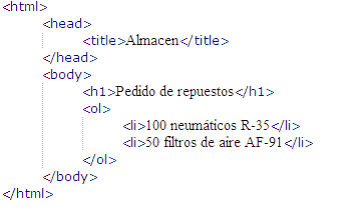
\includegraphics {figuras/png/EjemploHTML.png}

Si abrimos este fichero en un navegador cualquiera observamos lo siguiente:

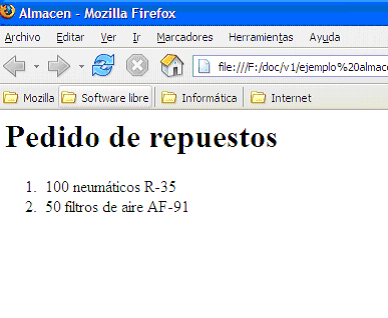
\includegraphics {figuras/png/Navegador.png}

Se puede abrir este ejemplo con cualquier otro navegador y se obtendr�a el mismo resultado (o al menos uno muy parecido) sin embargo no hay nada que indique que esto es un pedido, ni los elementos que se pide reponer, ni de qu� tipo son ni nada por el estilo y es que se debe recalcar que HTML es un lenguaje orientado a la presentaci�n.

Los elementos de marcado como <li>
solamente indican que una cadena de caracteres es un �tem de una lista pero ning�n programa que analizara el HTML de la Ilustraci�n 1  podr�a obtener ninguna informaci�n.

Existen mecanismos que permiten a�adir informaci�n sobre como se deben presentar las marcas en los navegadores pero en ning�n caso hay ninguna forma de separar el contenido de la presentaci�n, que es en suma el problema principal de HTML.

As�, XML surge como soluci�n a este problema al proponer un enfoque diferente a los propuestos por SGML y HTML.

\begin{itemize}
\item {XML es notablemente m�s sencillo que SGML por lo que el desarrollo de herramientas que lo usen se simplifica en gran medida.}
\item {XML no est� enfocado a la presentaci�n sino a contener informaci�n sobre la informaci�n marcada, es decir a servir de metainformaci�n. La presentaci�n de la informaci�n marcada mediante XML se har� mediante distintos lenguajes orientados a la presentaci�n de archivos XML.}
\end{itemize}

Este �ltimo punto es el que hace m�s atractivo a XML como formato de intercambio universal. XML permite marcar un documento con informaci�n que describa el contenido del archivo, sin indicar como se mostrar� y dejando la presentaci�n para otros lenguajes. Esta separaci�n de lenguajes es la que permite separar dos intereses encontrados como son la presentaci�n y el marcado del contenido.

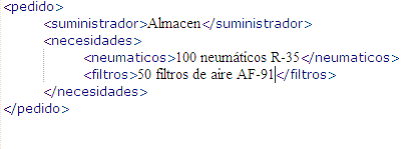
\includegraphics {figuras/png/EjemploXML.png}

En la Ilustraci�n 3 se muestra un ejemplo de c�mo se puede realizar el mismo documento anterior en XML aportando una cantidad de informaci�n mayor tanto al programa que necesite interpretar dicho fichero como a una persona que lo leyera.

Cabe destacar que XML no es un lenguaje en s� mismo sino un est�ndar que permite la definici�n de lenguajes propios mediante los criterios definidos en la especificaci�n de XML. Dicha especificaci�n es un documento p�blico y libremente accesible, desarrollado por el World Wide Web Consortium (o W3C) por lo que cualquier desarrollador o usuario puede implementar herramientas o documentos que sigan dicho est�ndar.

Existen multitud de tecnolog�as asociadas a XML encaminadas a definir est�ndares o a resolver problemas. Se citan a continuaci�n las que est�n mas avanzadas:

\begin{itemize}
\item {XML 1.0 y 1.1 son las recomendaciones  del W3C para construir documentos con marcas creadas por el usuario.}
\item {Las Definiciones de Tipo de Documento o DTD y los XML Schemas dictan las reglas a seguir para escribir las gram�ticas a las cuales se deben ce�ir los documentos XML. Se discutir�n las diferencias entre ellos m�s adelante.}
\item {Aparte de reglas para escribir documentos, el W3C publica normas para la construcci�n de bibliotecas que vayan a leer o escribir documentos XML. Estas normas indican los nombres de las clases, los m�todos, los interfaces y el comportamiento que deben tener las herramientas. Se hace una discusi�n m�s detallada en la p�gina 2 ("Implementaciones de APIs para XML") }
\item {XPath documenta las reglas a seguir para referirse a partes concretas de un documento.}
\item {CSS es un lenguaje heredado de HTML que permite escribir normas para que los documentos XML sean visibles en navegadores.}
\item {XSLT se usa para transformar un documento XML en otro documento XML que podr�a ce�irse a una gram�tica DTD distinta.}
\item {XSL:FO est� enfocada a convertir documentos XML en documentos imprimibles.}
\item {En XML hay una caracter�stica muy popular en los lenguajes de programaci�n denominada ``espacios de nombres'' y que permiten que marcas de uso com�n puedan repetirse en distintos documentos indicando que pertenecen a espacios distintos.}

\end {itemize}


\section {Implementaciones de APIs para XML}

A la hora de manipular documentos XML el W3C deseaba mantener todas las recomendaciones los m�s aisladas posible de ning�n lenguaje de programaci�n o compa��a concreta por lo que decidi� construir un est�ndar denominado DOM (Modelo de Objeto Documento).

El modelo de objeto documento describe una forma clara de manipular ficheros XML de acuerdo a una serie de reglas bien definidas y que respetan los principios de la orientaci�n a objetos. As�, un documento pasa a ser considerado un objeto con una serie de propiedades y m�todos y para el cual se definen una serie de interfaces que permiten su manipulaci�n.

Por ejemplo, en las recomendaciones del W3C se indica que debe existir un objeto que representa un elemento nodo y que se llamar� DOMNode. Adem�s dicho objeto debe tener una serie de m�todos como getChildNode() y que este m�todo devuelve un DOMNode que ser� el nodo hijo del elemento XML con el que se est� tratando. Este elemento DOMNode podr�a implementarse en C++, Java,  Visual Basic o C\#, pero lo verdaderamente importante es que el W3C publica todos los interfaces y cualquier desarrollador puede construir herramientas que implemente el est�ndar DOM con lo que se consigue un doble objetivo:

\begin {itemize}
\item {Por un lado, todos los desarrolladores pueden aprender f�cilmente a manejar nuevas bibliotecas que manipulen ficheros XML ya que conocen los mecanismos de funcionamientos, las clases y los m�todos que ofrecen.}
\item {Los creadores de bibliotecas pueden centrarse en construir aplicaciones eficientes al disponer de un an�lisis y un dise�o claros.}
\end {itemize}

A continuaci�n se describen con m�s detenimiento las principales APIs del W3C

\subsection{El API DOM}

DOM es un Interfaz


\subsection{El API SAX}

SAX es un Interfaz
\subsection{El API SAX}

SAX es un Interfaz
\subsection{Oracle XML-Dev Kit}

El kit de Oracle
\subsection{Xerces}

Xerces es una herramienta XML

\chapter {Desarrollo}
\section {An�lisis de las necesidades del usuario}
\section {Especificaci�n de requisitos software}
\section {Dise�o}

\subsection {Introducci�n}

En este apartado se define el dise�o del sistema en t�rminos de paquetes, clases, interrelaciones y comportamiento. Se utilizar�n diagramas UML para mostrar aspectos espec�ficos a destacar en el dise�o global del sistema como el dise�o de la interfaz de usuario o el dise�o estructural.

Existen algunos detalles importantes que un desarrollador deber�a conocer a la hora de entender, modificar o ampliar el dise�o sugerido:

\begin {itemize}

\item {La arquitectura global de la aplicaci�n est� basada en el patr�n Modelo-Vista-Control. Este patr�n muestra la soluci�n m�s cl�sica y eficaz para el desarrollo de una aplicaci�n interactiva separando claramente los componentes m�s elementales: Los datos que maneja la aplicaci�n (el ``Modelo''), los mecanismos que implementan la l�gica de control (el ``Controlador'' y el c�digo de la interfaz de usuario (la ``Vista'').}
\item {El Modelo no est� desarrollado mediante un lenguaje de programaci�n cl�sico, sino que consiste en la definici�n de un vocabulario XML que declara los componentes b�sicos necesarios para la automatizaci�n de un proceso, como por ejemplo rel�s, motores e interruptores.}
\item {El vocabulario del Modelo se especifica en un documento XML que contiene una definici�n escrita en XML Schema y donde se define la sintaxis que debe tener un modelo de sistema automatizado. La comprensi�n de la sintaxis del Schema puede resultar dif�cil para un desarrollador que se aproxime a ella por primera vez por lo que se recomienda leer la especificaci�n del World Wide Web Consortium para XML Schemas que se documenta en INSERTAR-----REFERENCIA----AQUI----- }
\item {El Controlador ha sido escrito en C++ est�ndar de forma que existe una correspondencia estricta entre los elementos definidos en el esquema y las clases que implementan un sistema. As� para cada elemento at�mico del esquema existe una clase que lo implementa.}
\item {Mantener la correspondencia entre una implementaci�n C++ y un documento XML que la represente es una tarea de gran complejidad. Por ello se ha utilizado Xerces, un framework escrito en C++ que implementa fielmente las recomendaciones del W3C para XML. Xerces posee implementaciones en C++ y Java, ademas de disponer de proyectos de implementaci�n en lenguajes alternativos.En ��INSERTAR REFERENCIA TUTORIAL WXWIDGETS AQUI!! se ilustra el uso de Xerces en un programa.}
\item {La Vista se ha implementado utilizando WxWidgets, un conjunto de clases multiplataforma para la escritura de interfaces de usuario altamente portable y con un aspecto diferenciado para los distintos sistemas de escritorio. La utilizaci�n de WxWidgets tambi�n presenta numerosas dificultades para un no iniciado por lo que su uso se describe con mayor amplitud en INSERTAR AQUI REFERENCIA TUTORIAL WXWIDGETS!!}
\item {La programaci�n del an�lisis de ficheros XML se puede hacer desde cero o utilizando las implementaciones de las recomendaciones del W3C. Estas recomendaciones especifican dos grandes enfoques de la programaci�n para XML, a saber: DOM y SAX. En este proyecto se ha utilizado la implementaci�n DOM de Xerces escrita en C+++}

\end {itemize}

El dise�o del software se ha centrado en la consecuci�n de una serie de objetivos:
\begin {itemize}
\item {Correcci�n: se pretende que el dise�o permita construir un programa que satisfaga los requisitos especificados.}
\item {Inteligibilidad: el dise�o no solamente es f�cil de transformar en una implementaci�n software sino que mediante el uso de patrones software deber�a ser f�cilmente comprensible para distintas personas que pretenden modificar o ampliar el sistema.}
\item {Modular: se ha intentado separar en capas los distintos aspectos concernientes a la implementaci�n de forma que las modificaciones supongan un impacto m�nimo, o al menos peque�o, en los distintos m�dulos.}
\item {Extensible: el uso de est�ndares bien conocidos as� como el aislamiento del c�digo en distintas capas debe facilitar la ampliaci�n del programa.}

\end {itemize}
\subsection {Dise�o estructural}
A continuaci�n se muestra el diagrama de la arquitectura global de la aplicaci�n:

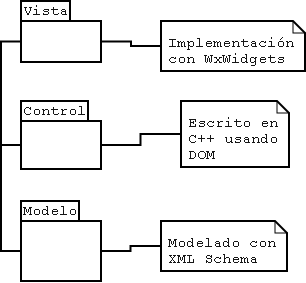
\includegraphics {figuras/png/Arquitectura.png}

La arquitectura MVC permite un desacoplamiento entre los distintos objetos que componen el sistema, permitiendo minimizar el impacto de los cambios entre capas del software. Adem�s, supone una arquitectura bien conocida, f�cil de entender, con riesgos calculados y que facilita la implementaci�n en un lenguaje dado, laportabilidad y las modificaciones.

Adem�s, la elecci�n de una arquitectura MVC no solo fomenta el desarrollo modular del programa sino que tambi�n expone claramente dicha modularidad, facilitando as� la comprensi�n del programa por parte de futuros desarrolladores. La estructura de dichos m�dulos se explicar� en subsiguientes p�rrafos.

El software se ha desarrollado como una aplicaci�n de escritorio 
monoproceso, pensada para ejecutarse en un entorno gr�fico. No se debe confundir la arquitectura MVC con las cl�sicas aplicaciones Web de 3 capas donde existen 3 procesos distintos que se ejecutan en tres nodos distintos a saber: El navegador Web que muestra la p�gina HTML, el servidor que atiende las peticiones HTML y de datos y el servidor de bases de datos que almacena y entrega los datos bajo petici�n del servidor Web. El programa tambi�n utiliza 3 capas, una de presentaci�n, una de l�gica de control y una de almacenamiento pero su prop�sito principal es la modularidad, y no la ejecuci�n separada de los distintos procesos.

A continuaci�n se muestran los componentes principales de cada capa:

Capa de Interfaz de usuario

Capa de control

Capa de modelo

Debido a la simplicidad de su arquitectura el despliegue de la misma no debe suponer ning�n problema, al haberse pensado la misma para construir un �nico programa ejecutable dependiente de algunas bibliotecas y que se ubicar� mediante un instalador en el directorio seleccionado por el usuario. En el manual de uso se describir� m�s ampliamente el proceso de despliegue. Las distintas capas de esta arquitectura han presentado ciertos problemas a la hora de su desarrollo ya que algunos problemas no se conoc�an en las etapas iniciales, como por ejemplo la integraci�n entre los distintos tipos de cadena de caracteres que ofrecen las distintas bibliotecas usadas al codificar.

La integraci�n de nuevos componentes 





\section {Implementaci�n}
\section {Pruebas}

\subsection {Formato de las pruebas}
\subsection {Casos de prueba}

\subsection {Las herramientas xUnit para la prueba de software}

Las pruebas de unidad son un tipo de pruebas que en los �ltimos tiempos han alcanzado una gran popularidad en el desarrollo de programas. Tradicionalmente el ciclo de vida de los programas ha venido caracteriz�ndose por las fases enumeradas y secuenciadas en la 


\chapter {Resultados}
\chapter {Propuestas}

Nada todav�a

%A partir de aqui van los ap�ndices
\appendix


%\chapter {Referencia r�pida de WxWidgets}

\section {Un primer programa}

Un programa en WxWidgets solo se puede lanzar desde dentro de una clase especial por lo que para empezar se debe crear una clase que herede de esta clase llamada wxApp y que por ejemplo llamaremos Aplicaci�n. Dentro de esta clase se pueden implementar todos los m�todos que queramos pero sobre todo se debe implementar un m�todo virtual que proporciona wxApp y cuya declaraci�n es la siguiente:

\begin{lstlisting}
virtual bool OnInit()
\end{lstlisting}
Normalmente dentro de OnInit crearemos la ventana principal del programa pero sobre todo debemos terminar devolviendo un valor bool que indique a wxWidgets si debe comenzar o no el bucle de procesado de eventos, por lo que a no ser que se desee algo muy especial se devolver� true la mayor parte de las veces.

Es posible preguntarse �donde est� la funci�n main() o WinMain o el punto de entrada al programa?. En ning�n sitio, no se debe poner pues WxWidgets lo a�ade autom�ticamente. Lo �nico que necesita saber la biblioteca es el nombre de la clase que tiene que asignar a un objeto interno denominado wxTheApp (que normalmente no es necesario manipular) y para indic�rselo se usa la macro

\begin{lstlisting}
DECLARE_APP (<nombre de la clase que hereda de wxApp>)
\end{lstlisting}

Para que la funci�n pueda enlazar el m�todo OnInit al punto de entrada al programa se debe utilizar la macro 

\begin{lstlisting}
IMPLEMENT_APP (<nombre de la clase que hereda de wxApp>)
\end{lstlisting}

As�, una clase Aplicaci�n muy simple ser�a como la siguiente:

\begin{lstlisting}

// Este es el fichero de cabecera aplicacion.h
\#include "wx/wx.h"

class Aplicacion : public wxApp
{
 public:
   virtual bool OnInit(); 
};

DECLARE_APP (Aplicacion)


\end{lstlisting}

\begin{lstlisting}

//Este es el fichero aplicacion.cpp

#include "aplicacion.h"
#include "ventana.h"

IMPLEMENT_APP (Aplicacion)

bool Aplicacion::OnInit()
{
  Ventana *v=new Ventana();
  v->Show(true);
	return (true);
}

\end{lstlisting}

Como se puede ver, lo �nico que hace el m�todo OnInit es crear un objeto de la clase Ventana (que se comentar� en seguida) y llamar a su m�todo Show, devolviendo true al final y comenzando as� el bucle de eventos.

Todo esto por s� mismo no hace nada. Una biblioteca para construcci�n de interfaces de usuario debe proporcionar mucho m�s. Para empezar, veamos como crear una simple ventana. Existen muchas clases de ventana pero la m�s elemental es wxFrame, que contiene el comportamiento m�s b�sico de cualquier ventana. Hay que destacar que en wxWidgets se permite un control total sobre el comportamiento de TODOS los controles por lo que la complejidad de la programaci�n con esta biblioteca tambi�n es muy grande. Sin embargo una vez superada la curva de aprendizaje se dispone del control total sobre el m�s m�nimo detalle sumado a la ventajas de la programaci�n multiplataforma.

Empezaremos creando una ventana muy simple. Para ello crearemos una clase Ventana que herede de wxFrame

\begin{lstlisting}
// Fichero ventana.h
#include "wx/wx.h"

class Ventana : public wxFrame
{
 public:
  Ventana();
};

\end{lstlisting}

Cuya implementaci�n se muestra en el siguiente fichero

\begin{lstlisting}
//Fichero ventana.cpp

#include "ventana.h"

Ventana::Ventana() :
 wxFrame (NULL, wxID_ANY, "Ventana con WxWidgets")
{
}

\end{lstlisting}

Como se puede ver, lo �nico que se hace es llamar al constructor de la clase padre. Se pueden pasar muchos par�metros (consultar la ayuda de WxWidgets para ampliar) pero con los tres primeros es suficiente. El primer par�metro pide el identificador de ventana de la ventana ``padre'' de esta ventana. Si se desea que �sta sea la ventana principal pasamos NULL. El segundo par�metro permite indicar el identificador de esta ventana. Usando la constante predefinida wxID\_ANY permitimos que la biblioteca asigne cualquiera que est� libre. El tercer par�metro es el t�tulo que debe aparecer en la ventana.

Aparte de eso, no se hace absolutamente nada m�s. En la clase principal aplicaci�n se cre� un objeto ventana y se llam� al m�todo Show() que mostrar� esta ventana principal. Si compilamos y ejecutamos obtendremos una ventana como la siguiente:

\begin{figure}
	\begin{center}
		
\includegraphics[scale=0.45]{figuras/png/ventanasimple.png}
	\end{center}
	\caption{Ventana m�nima de WxWidgets}
	\label{fig:ventanasimple}
\end{figure}


Esta ventana se puede mover, cerrar, cambiar de tama�o etc... y sin haber programado nada. La clase wxFrame proporciona el comportamiento por defecto para una ventana est�ndar

Sin embargo una ventana vac�a no sirve de mucho. Una aplicaci�n normal constar� de botones, cuadros de texto, men�s, etc... Y aqu� entra otro concepto fundamental en WxWidgets. Los eventos. En todas las bibliotecas orientadas a la programaci�n gr�fica existe el concepto de funciones que se disparan cuando se produce un evento y que se denominan funciones de retro-llamada o funciones callback. En WxWidgets se deben declarar cuales son las funciones que se disparan cuando se produzca un cierto evento y conectar esas funciones a eventos concretos. Una ventana o control que desee responder a eventos deber� incluir la macro DECLARE\_EVENT\_TABLE en su fichero de declaraci�n (en este caso ventana.h) y macros que conecten los eventos (identificados por un n�mero que declararemos m�s adelante) a dichas funciones. Esta conexi�n se suele hacer en el fichero de implementaci�n (ventana.cpp) y usando las macros BEGIN\_EVENT\_TABLE() y END\_EVENT\_TABLE()
Por ejemplo, supongamos que queremos que nuestra ventana reaccione a la pulsaci�n de la tecla C y que su reacci�n consista en cerrar la ventana. Para ello, hay que crear una funci�n callback en la clase Ventana como esta

\begin{lstlisting}
void OnPulsaTecla (wxKeyEvent &evento); 
\end{lstlisting}

La clase wxKeyEvent almacena un evento de pulsaci�n de tecla. No necesitamos manejarla ya que el bucle de eventos nos entregar� dicho evento de pulsaci�n en la aplicaci�n.

Su implementaci�n comprueba si se ha pulsado la C
\begin{lstlisting}
void OnPulsaTecla (wxKeyEvent &evento)
{
 //Se comprueba si el c�digo ASCII de la tecla pulsada es C
 if (evento->m_keyCode == 67)
 {
  Close();
 }
}
\end{lstlisting}

Y se conecta el evento de pulsaci�n de teclado a esta funci�n con
\begin{lstlisting}
BEGIN_EVENT_TABLE(Ventana, wxFrame)
 EVT_KEY_DOWN (Ventana::OnPulsaTecla)
END_EVENT_TABLE()
\end{lstlisting}

Por lo que el fichero ventana.h queda
\begin{lstlisting}
#include "wx/wx.h"

class Ventana : public wxFrame
{
 public:
  Ventana();
	void OnPulsaTecla (wxKeyEvent &evento);
 private:
  DECLARE_EVENT_TABLE ()
};
\end{lstlisting}

y el fichero ventana.cpp queda

\begin{lstlisting}
#include "ventana.h"

Ventana::Ventana() :
 wxFrame (NULL, wxID_ANY, "Ventana")
{
}


void Ventana::OnPulsaTecla (wxKeyEvent &evento)
{
 //Se comprueba si el c�digo ASCII de la tecla pulsada es C
 if (evento.m_keyCode == 67)
 {
  this->Close();
 }
}

BEGIN_EVENT_TABLE(Ventana, wxFrame)
 EVT_KEY_DOWN (Ventana::OnPulsaTecla)
END_EVENT_TABLE()

\end{lstlisting}


Sizers

Los sizer son ``ajustadores de tama�o''. Son elementos corrientes en la programaci�n gr�fica y sobre todo en la multiplataforma, existen en GTK, en QT, en Java y en otros toolkits menos populares como FLTK, etc... La idea de un sizer es almacenar controles gr�ficos ajustando el tama�o de lo que contienen. En principio podr�amos desear que los botones, paneles o men�s tuvieran un tama�o fijo pero esto no es buena idea debido a las variaciones de resoluci�n de unos sistemas a otros por un lado y a la posibilidad de poder reajustar autom�ticamente el tama�o de los controles si alguien cambia el tama�o de la ventana. Un sizer se limita a almacenar controles y calcular autom�ticamente el mejor tama�o, manteniendo la proporcionalidad si queremos por supuesto. El algoritmo de c�lculo de tama�o de un control se basa en si hay controles hijo y en el tama�o total de la ventana (ya que puede haber otros sizers conteniendo m�s controles) y es bastante complejo. No se necesitan saber los detalles pero se puede acudir a la documentaci�n de WxWidgets si se desea m�s informaci�n. Para nuestros intereses pensemos simplemente que los sizer son ``contenedores invisibles'' y que ajustan el tama�o autom�ticamente. 

Existen varios tipos de sizer: Contenedores que ajustan los controles horizontalmente, verticalmente, en rejilla, etc... Al utilizar los distintos sizer se debe de olvidar el concepto de que un bot�n mide x p�xeles y otro bot�n mide y p�xeles. Al usar contenedores como los sizer solo se necesita pensar en el ``tama�o relativo''. Por ejemplo, supongamos que deseamos que en nuestra ventana haya dos botones y un control de texto. Cuando se pulse uno de los botones se imprimir� un mensaje en el control de texto y al pulsar el otro se imprime un mensaje distinto. Si deseamos que el control de texto ocupe la mitad superior y el par de botones la mitad inferior podr�amos pensar en apilar los controles. Esto se puede hacer mediante un wxBoxSizer, que se limita a poner los controles uno detr�s de otro en horizontal (pasando el par�metro wxHORIZONTAL) o poniendo uno debajo de otro (usando wxVERTICAL)

Para conseguir esto, a grandes rasgos solo tenemos que crear el contenedor, crear los tres controles, a�adir los controles al contenedor y hacer que el contenedor sea el contenedor principal de nuestra ventana. As� que en el fichero ventana.cpp la implementaci�n del constructor queda as�:

\begin{lstlisting}
Fichero ventana.cpp
Ventana::Ventana() :
 wxFrame (NULL, wxID_ANY, "Ventana")
{
 contenedor= new wxBoxSizer(wxVERTICAL);
 boton1 = new wxButton (this, wxID_BOTON1, "Mensaje 1");
 boton2 = new wxButton (this, wxID_BOTON2, "Mensaje 2");
 texto = new wxTextCtrl(this, wxID_ANY, "Aqui va el texto",
 wxDefaultPosition, wxDefaultSize, wxTE_MULTILINE);
 contenedor->Add (boton1);
 contenedor->Add (boton2);
 contenedor->Add (texto);
 this->SetSizer (contenedor);
}
\end{lstlisting}

Si compilamos veremos que se obtiene algo semejante a esto:

INSERTAR AQUI IMAGEN SIZER

Se observan varias cosas

\begin{itemize}
	\item {
		Aunque se pulsen los botones no pasa nada.
	}
	\item {
		Los controles est�n demasiado pegados.
	}
	\item {
		La apariencia de los controles no es la que esper�bamos.
	}

\end{itemize}

En cuanto al primer problema la respuesta es simple. Tenemos que gestionar los eventos de pulsaci�n y conectarlos con funciones que impriman cosas en el control. El segundo y el tercer problema tienen que ver con los contenedores y su gesti�n Para resolver el primer problema simplemente creamos una funci�n como esta en el fichero de implementaci�n

\begin{lstlisting}
void Ventana::OnPulsacionBoton1(wxCommandEvent& evento)
{
 texto->AppendText ("Se ha pulsado el boton 1\n");
}
\end{lstlisting}

Y conectamos el evento de pulsaci�n de bot�n con esta funci�n


\begin{lstlisting}
BEGIN_EVENT_TABLE(Ventana, wxFrame)
 EVT_KEY_UP (Ventana::OnPulsaTecla)
 EVT_BUTTON (wxID_BOTON1, Ventana::OnPulsacionBoton1)
END_EVENT_TABLE()
\end{lstlisting}

De forma que el fichero ventana.h queda as�

\begin{lstlisting}
#include "wx/wx.h"

class Ventana : public wxFrame
{
 public:
  Ventana();
	void OnPulsaTecla (wxKeyEvent &evento);
	void OnPulsacionBoton1(wxCommandEvent& evento);
	void OnPulsacionBoton2(wxCommandEvent& evento);
 private:
  wxBoxSizer* contenedor;
  wxButton* boton1;
  wxButton* boton2;
  wxTextCtrl* texto;
  DECLARE_EVENT_TABLE ()
};

enum {
 wxID_BOTON1=1,
 wxID_BOTON2=2
}
}; //Fin de la clase

\end{lstlisting}

Y ventana.cpp contiene:

\begin{lstlisting}
#include "ventana.h"

Ventana::Ventana() :
 wxFrame (NULL, wxID_ANY, "Ventana")
{
 /* Se crea el contenedor */
 contenedor= new wxBoxSizer(wxVERTICAL);
 
 /* Se crean los controles*/
 boton1 = new wxButton (this, wxID_BOTON1, "Mensaje 1");
 boton2 = new wxButton (this, wxID_BOTON2, "Mensaje 2");
 texto = new wxTextCtrl(this, wxID_ANY, "Aqui va el texto",
 wxDefaultPosition, wxDefaultSize, wxTE_MULTILINE);

 /* Se a�aden los controles*/
 contenedor->Add (boton1);
 contenedor->Add (boton2);
 contenedor->Add (texto);
 
 /* Y se establece el contenedor*/ 
 this->SetSizer (contenedor);
}

void Ventana::OnPulsaTecla (wxKeyEvent &evento)
{
 //Se comprueba si el c�digo ASCII de la tecla pulsada es C
 if (evento.m_keyCode == 67)
 {
  this->Close();
 }	
}

void Ventana::OnPulsacionBoton1(wxCommandEvent& evento)
{
 texto->AppendText ("Se ha pulsado el boton 1\n");
}

BEGIN_EVENT_TABLE(Ventana, wxFrame)
 EVT_KEY_UP (Ventana::OnPulsaTecla)
 EVT_BUTTON (wxID_BOTON1, Ventana::OnPulsacionBoton1)
END_EVENT_TABLE()

\end{lstlisting}

Con esto, al pulsar el primer boton se a�ade un mensaje control de texto. 

El siguiente problema es algo m�s dif�cil de resolver, �Como conseguir que los controles tengan la apariencia que queremos?. En primer lugar, nos gustar�a que los botones estuvieran centrados horizontalmente. Si miramos la documentaci�n veremos que se puede a�adir el flag wxALIGN\_CENTER al m�todo Add del contenedor, que los centrar�. As� que las l�neas de a�adido quedan as�

\begin{lstlisting}
contenedor->Add (boton1, wxALIGN_CENTER);
contenedor->Add (boton2, wxALIGN_CENTER);
\end{lstlisting}

Y se obtiene


INSERTAR AQUI LA IMAGEN DE LOS SIZER

La explicaci�n a esto es que el contenedor est� poniendo controles UNOS ENCIMA DE OTROS por lo que al centrar se dedica a centrar VERTICALMENTE. La soluci�n al problema pasa por las jerarqu�as de contenedores. Los botones ir�n en su propio wxBoxSizer en horizontal, y dichos contenedores se pondran unos encima de otros. Los contenedores de los botones alinear�n en horizontal y esos ``alineadores horizontales'' deben ir ``alineados verticalmente'' unos encima de otros.

As�, habr� un contenedor para los botones que ir� en la parte superior y otro para el control de texto que ir� en la parte inferior. Cuando a�adamos los botones al contenedor podemos especificar el flag wxALIGN\_CENTER que centrar� el bot�n horizontal y verticalmente dentro del contenedor, y si usamos el flag wxALL a la vez que especificamos un tama�o de borde podremos poner ese borde de distancia entre el bot�n y los controles que est�n en todas partes (se podr�a poner distancia solo por la izquierda por ejemplo con wxLEFT).

Otro concepto importante que se da al a�adir un control a un contenedor es la proporci�n. Si especificamos una proporci�n distinta de 0 al a�adir un control estamos permitiendo que ese control ocupe m�s espacio relativo dentro de un contenedor. Si por ejemplo se a�aden 3 botones y uno de ellos se a�ade con proporcion 1, obtendr� m�s espacio para ``agrandarse'' que los dem�s.

Si miramos la nueva implementaci�n de ventana.cpp


\begin{lstlisting}
#include "ventana.h"

Ventana::Ventana() :
 wxFrame (NULL, wxID_ANY, "Ventana")
{
 /* Se crea el contenedor */
 contenedor= new wxBoxSizer(wxVERTICAL);
 
 /* Se crean los contenedores de los botones*/
 contenedorBotones = new wxBoxSizer (wxVERTICAL);
 /* Se crean los controles*/ 
 boton1 = new wxButton (this, wxID_BOTON1, "Mensaje 1");
 boton2 = new wxButton (this, wxID_BOTON2, "Mensaje 2");
 texto = new wxTextCtrl(this, wxID_ANY, "Aqui va el texto",
  wxDefaultPosition, wxSize (180,60), wxTE_MULTILINE);
	
 /*Se a�aden los controles con 10 pixeles de borde por todos
 los lados y alineados horizontal y verticalmente.
 Los dos usan la misma proporci�n (0) por lo que 
 conservan su proporcion dentro de contenedorBotones*/

 contenedorBotones->Add(boton1,0, wxALL | wxALIGN_CENTER, 10);
 contenedorBotones->Add(boton2,0, wxALL | wxALIGN_CENTER, 10);
 
 /* Se a�aden al contenedor principal la botonera y 
 el control de texto. El control de texto puede expandirse
 hacia los lados (ya que la gesti�n vertical la realiza
 su contenedor) y adem�s ocupa mayor proporcion que 
 los botones */
 contenedor->Add (contenedorBotones,0, wxALIGN_CENTER);
 contenedor->Add (texto, 1, wxEXPAND);
	
 /* Y se establece el contenedor*/
 this->SetSizer (contenedor);

 /* El contenedor se ensancha hasta ocupar 
 el �rea de la ventana */
 contenedor->Fit (this);

 /* Y la ventana regir� su tama�o m�nimo por el de
  este contenedor */
 contenedor->SetSizeHints (this);
}

\end{lstlisting}


\bibliography{bibliografia/bibliografia}\bibliographystyle{alpha}
\end {document}
